\documentclass{article}
\usepackage[utf8]{inputenc}
\usepackage{graphicx}
\usepackage{listings}
\usepackage{graphicx}
\usepackage{tabularx}

\title{Recommender Systems: Predicting Probabilistic Rating from User ID and Item ID in R}

\author{Leo Martinez-Perez\\
    \texttt{leomartinezp@ucdavis.edu}
    \and Member 2\\
    \texttt{member2@ucdavis.edu}
    \and Member 3\\
    \texttt{member3@ucdavis.edu}
    \and Member 4\\
    \texttt{member4@ucdavis.edu}
    \and Member 5\\
    \texttt{member5@ucdavis.edu}
}

\date{March, 2020}

\begin{document}

\maketitle

\newpage
\section{Logit}

\subsection{Introduction to the Logistic Regression Model}

In classification problems, one often wishes to predict whether or not a collection of data pertains to a specific category. In order to achieve this, we can use a logistic regression model to predict the mean of a binomially distributed indicator variable that indicates whether the data belongs to the category. This mean will be within the range [0,1] and represent the probability that the variable will be equal to 1. In our case our indicator variables will be whether or not the user gave the item the rating r, where r represents all possible ratings that could be given to the item. 

$\newline$
This method utilizes the logistic function, $\frac{1}{1+e^{-\mu}}$, where $\mu$ is a model of the different users and items multiplied by linear parameters, $\beta_0 + \beta_1x_1 + ... + \beta_nx_n$. These parameters can be estimated iteratively through the Maximum Likelihood Estimation method by being exposed to a set of training data. 

\subsection{Usage of the 'logit' Prediction Method}
The ratingsProbsFit function can generate estimates of the probability that users would rate certain items different ratings using a logistic regression model. In order to do this one must pass the string 'logit' in place for predMethod under the function call: 

\begin{lstlisting}[language=R]
ratingProbsFit(dataIn,maxRating,predMethod,embedMeans,
specialArgs)
\end{lstlisting}

$\newline$
In the case of logit, dataIn must be preprocessed before hand and the first two columns must be names userID and itemID respectively, while the third column must represent the rating, embedMeans can be turned either on or off, and specialArgs will be discarded. 

\subsection{Implementation of Logit}
Logit was implemented by using the built-in R function "glm". Glm stands for generalized linear models and supports several parametric families. In order to use logit we must specify to use the binomial family. The implementation of our code draws inspiration from the One vs. All method. The One vs. All method is used when one is attempting to categorize something that could belong to one of several categories. In order to determine a prediction for which category the data belongs to, we can create a separate model for every single category and categorize it corresponding to whichever model yields the most certain prediction. In our case, however, we are not attempting to categorize the data. Therefore we can simply generate n different models, where n is the number of possible ratings. We can then return these models inside of an R S3 object or a list.

$\newline$
This object can then generate the probabilities that the a given user would rate a given movie a certain rating by using the built-in R function 'predict'. Predict.glm takes in a general linear model, the new data to predict, and the optional parameter of type = 'response', which indicates to the function that the prediction should be a probability. In order to generate the probabilities for every possible rating, we must call predict for every single glm model that was generated from the ratingProbsFit function.

\subsection{Shortcomings of Logit}
During the exploration of the Logit method for classification, we encountered a couple of shortcomings that make it difficult to use Logit in every situation.

$\newline$
A common question asked in computer science is, "does it scale"? Unfortunately, when testing our implementation of Logit one of the first issues we noticed was that the time complexity to generate logistic regression models for every possible rating was very large. When handling data points like userID and itemID with many factors, glm must create dummy variables for every single level. As a result, it would take approximately thirty minutes to finish computing the probabilities for a data set of 10,000 rows on our personal computers. Assuming a linear increase in time as we increased the number of rows, to run glm on a dataset of a million rows it would take us 50 hours. 

$\newline$
Another issue with using Logit for classification is that it does not account for new users or items. If the training model has not been exposed to a user or an item when attempting to predict it will not know what to do. As a result, if you wished to introduce new users or items you would have to recompute the entire model. On a similar note, one must be extremely careful when partitioning the data into a training set and testing set during cross validation for Logit. This is because, one must ensure that every item and movie within the testing set is present in the training set. 

\subsection{Testing the Effectiveness of Logit}
\subsubsection{InstEval Data Set}
The first data set which we used to test Logit was the InstEval data set. The InstEval data set represents a collection of students, instructors, and ratings of the lecturers from one to five. Due to the scale of the data set, we decided to trim the data set such that only the first 10,000 rows are used. In order to partition these 10,000 rows into a training and testing set we used an algorithm found on Stack Overflow (https://stackoverflow.com/questions/19946930/r-cross-validation-on-a-dataset-with-factors) by user musically\_ut. The following section of code demonstrates the code used to generate the partition.

\begin{lstlisting}[language=R]
  test <- setdiff(1:nrow(dataIn), train)

  n <- floor(0.95 * nrow(dataIn))
  cond <- FALSE
  
  while(!cond) {

    trainIndx <- sample(nrow(dataIn), n)
    testIndx <- setdiff(1:nrow(dataIn), trainIndx)
    cond <- TRUE

    for(factor in names(dataIn)[1:2]) {
      trainLevels <- dataIn[trainIndx, factor]
      testLevels <- dataIn[testIndx, factor]
      
      if(!all(testLevels %in% trainLevels)) {
        cond <- FALSE
      }
    }
  }
\end{lstlisting}

$\newline$
This code takes a random sample of 95\% of the total data for the training set and the remaining 5\% for the testing set. It then checks to see if the testing set is a subset of the training set. If it isn't it creates another random partition of the data and checks again until it is valid. 

$\newline$
After using this partition to determine the probabilities of each possible rating, we can save the data set to a file in order to analyze it. One of the first things we did to verify the validity of our data set was to ensure that every row added up to one and thus represented a complete view of all the possible ratings that could occur. In our case it added up to approximately one. We attributed this to rounding errors with the significant figures reported by R.

\begin{figure}[h!]
\centering
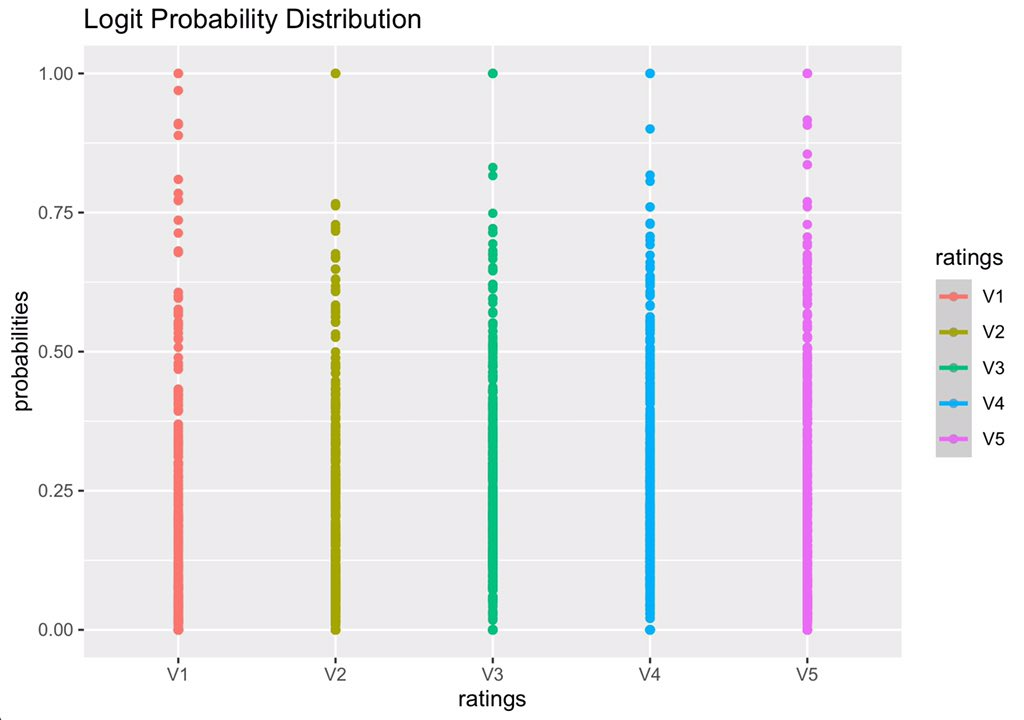
\includegraphics[scale=0.25]{LogitProbDistribution.jpg}
\caption{Logit Probability Distribution}
\label{fig:universe}
\end{figure}

$\newline$
In order to analyze the probabilities outputted by Logit, we decided to plot the probabilities such that it would reflect a probability distribution of all the ratings (Figure 1: Logit Probability Distribution). From first glance, we can notice that there are some probabilities that were automatically fitted to be zero or one. This can be seen in the points which lie on the probabilities = 1 axis. We suspect that this may be because of outliers in our data. If one wanted to explore deeper into this, they could make note of the userIDs and itemIDs that are generating fitted probabilities. They could then extract the glm objects outputted by ratingProbsFit and analyze the standard error reported for those userIDs and itemIDs. 

$\newline$
We also noted that the probability distribution somewhat resembled that of a binomial distribution graph generated by a histogram. This is because there appears to be a peak at a rating of three and as the rating strays from the peak its probability is reduced on average. This is what we expected to see because we generated the linear regression such that the rating modeled a binomial distribution.

$\newline$
The raw output of the probabilities can be found in the LogitPredictions.data file submitted with this project. The LogitPredictions.data are the probabilities predicted from the TrimmedTest.data file after training our model on the TrimmedTrain.data.

\subsubsection{Song List Data Set}
The second data set which we used test Logit was the Song List data set. The Song List data set represents a collection of users, songs, and the ratings of those songs from one to five. Much like the InstEval data set we opted to only use the first 10,000 rows of the data set and we partitioned it using a 95\%/5\% split. However, our algorithm was unable to find a successful partition after about an hour of attempts. This prompted a deeper look at the code that we were analyzing. We noticed that there were 200,000 unique users and 127,771 unique songs within this data set. Therefore we increased our data set to be first 100,000 rows of the original data set. In this case, we were also unable to find a successful partition after attempting to do so for a long time. We could greatly increase our chances of finding a successful partition if we were to increase the size of the data we were using. However, the computation of the probabilities would be unfeasible to run on our personal computers. As a result we were forced to omit the analysis of the probabilities produced by Logit on the Song List data set. 

\section{Who Did What?}
\subsection{Leo Martinez-Perez}
Leo worked on the Logit component of this project. This includes the research, implementation, testing, and write up for the Logit method. In addition to this, Leo participated in the group discussions and helped discuss ideas for other implementations with the other group members. 
\end{document}
